% -----------------------------------------------
% Template for ISMIR 2014
% (based on earlier ISMIR templates)
% -----------------------------------------------

\documentclass{article}
\usepackage{ismir2014,amsmath,cite}
\usepackage{graphicx}
\usepackage{brian}

% Title.
% ------
\title{Analyzing song structure with spectral clustering}

% Single address
% To use with only one author or several with the same address
% ---------------
%\oneauthor
% {Names should be omitted for double-blind reviewing}
% {Affiliations should be omitted for double-blind reviewing}

% Two addresses
% --------------
%\twoauthors
%  {First author} {School \\ Department}
%  {Second author} {Company \\ Address}

% Three addresses
% --------------
\threeauthors
  {First author} {Affiliation1 \\ {\tt author1@ismir.edu}}
  {Second author} {\bf Retain these fake authors in\\\bf submission to preserve the formatting}
  {Third author} {Affiliation3 \\ {\tt author3@ismir.edu}}

% Four addresses
% --------------
%\fourauthors
%  {First author} {Affiliation1 \\ {\tt author1@ismir.edu}}
%  {Second author}{Affiliation2 \\ {\tt author2@ismir.edu}}
%  {Third author} {Affiliation3 \\ {\tt author3@ismir.edu}}
%  {Fourth author} {Affiliation4 \\ {\tt author4@ismir.edu}}

\begin{document}
%
\maketitle
%
\begin{abstract}
Many approaches to analyzing the structure of a musical recording involve detecting
sequential patterns within a self-similarity matrix derived from time-series features.
Such patterns ideally capture repeated sequences, which then form the building blocks
of large-scale structure.

In this work, we apply techniques from spectral graph theory to analyze repeated
patterns in musical recordings.  The proposed method produces a low-dimensional
encoding of repetition structure, and exposes the hierarchical relationships among
structural components at differing levels of granularity.
\end{abstract}
%
\section{Introduction}\label{sec:introduction}

\subsection{Our contributions}

\subsection{Related work}

\cite{mauch2009using}

\cite{serra2012unsupervised}

\cite{grohganz2013converting}

\section{Encoding repetition}
% Begin with nearest-neighbor linkage in some feature space
% Apply diagonal majority vote filtering
% Add the conveyor belt links
% Compute the graph laplacian, observe magic

Let $X = [x_1, x_2, \dots, x_n] \in \R^{d\times n}$ denote a $d$-dimensional time
series feature matrix, \eg, a chromagram or sequence of Mel-frequency cepstral 
coefficients).  As a first step toward detecting and representing repetition structure, 
we form a \emph{binary recurrence matrix} $R \in \{0,1\}^{n\times n}$, where 
\begin{equation}
R_{ij}(X) \defeq \begin{cases}
1 & x_i, x_j \text{ are mutual $k$-nearest neighbors}\\
0 & \text{otherwise},
\end{cases}
\end{equation}
where $k$ is a linkage parameter controlling the degree of connectivity in $R$.

% FIXME: cite for recurrence matrix

If $X$ sufficiently captures the qualities of interest, and $k$ is large
enough, then repeated structures should appear as diagonal stripes in $R$.
In practice, it is beneficial to apply a smoothing filter to $R$ to suppress erroneous
links, and fill in gaps.  Here, we apply a windowed majority vote to each diagonal of
$R$, resulting in the filtered matrix $R'$:
\begin{equation}
R'_{ij} \defeq \maj\left\{ R_{i-w, j-w}, \dots, R_{i+w, j+w}\right\},
\label{filtered-rep}
\end{equation}
where $w$ is a discrete parameter that defines the minimum length of a valid
repetition sequence.

The filtered recurrence matrix $R'$ can be interpreted as an unweighted, undirected 
graph, whose vertices correspond to samples (columns of $X$), and edges correspond 
to equivalent position within a repeated sequence. Note, however, that successive 
positions $(i, i+1)$ will not in general be connected in $R'$, so the constituent 
samples of a particular sequence will not be directly linked.

In order to facilitate the discovery of repeated sections, we modify $R'$ by 
adding links between adjacent samples $(i, i+1)$ and $(i, i-1)$, resulting in the
\emph{sequence-augmented graph} $R^+$:
\begin{equation}
R^+_{ij} \defeq \begin{cases}
1 & |i - j| = 1\\
R'_{ij} & \text{otherwise}.
\end{cases}\label{pathmatrix}
\end{equation}
With appropriate normalization, $R^+$ can be interpreted as a Markov process
over samples, where at each step $i$, the process either moves to an adjacent
sample $i\pm1$, or a random repetition of $i$; a process exemplified by the 
Infinite Jukebox~\cite{infinitejukebox}.

\Cref{pathmatrix} explicitly combines local temporal connectivity with long-term
recurrence information.  Ideally, we would add connections only to pairs $\{i,j\}$
belonging to the same component, but of course, this information is hidden.  Rather,
by adding links along the first diagonals, the graph becomes fully connected.  
However, repeated sections will contain internal connectivity structure.  Let $i$ and
$j$ denote two repetitions of the same sample at different times; then $R^+$ should
ideally contain edges $\{i, i+1\}$, $\{i, j\}$, $\{i+1, j+1\}$, $\{j, j+1\}$.
Connections between unrelated blocks are likely to remain sparse, owing primarily to
cross-section links along the first diagonals.  

% For the purposes of musical structure analysis, we would like to produce a block
% matrix $C$, where $C_{i,j}$ indicates that $i$ and $j$ belong to the same structural
% component (\eg, $i$ and $j$ are both of type \emph{verse}).

\subsection{Spectral clustering}

The Laplacian is a fundamental tool in the field of spectral graph
theory, as its spectrum can be used to characterize 
connectivity among vertices~\cite{chung1997spectral}.  
Let $A$ denote the adjacency matrix of \cref{pathmatrix}, and define $D$ as the
diagonal \emph{degree matrix}: $D \defeq \diag(\sum_{j} A_{\cdot, j})$.  The
\emph{random-walk normalized Laplacian} $L$ is defined as:\footnote{Other forms of
Laplacian normalization are commonly used in practice.  We selected random-walk
normalization according to the motivations described by 
von~Luxburg~\cite{von2007tutorial}.}
\begin{equation}
L \defeq D^{-1} (D - A) = I - D^{-1} A.\label{rwlaplacian}
\end{equation}

The Laplacian forms the basis of spectral clustering~\cite{von2007tutorial}.  The
motivation for its use stems from the observation that the multiplicity of the bottom
eigenvalue $\lambda_0 = 0$ corresponds to the number of connected components in a
graph, and the corresponding eigenvectors $y_i \in \R^n$ encode membership of vertices
in components.

In the non-ideal case --- as we have with $A$ --- the graph is fully connected, and
the bottom eigenvector $y_0$ is a constant vector which trivially encodes membership 
in the graph.  However, in the case of $A$, we expect there to be many components
with relatively small inter-connectivity, \ie, when one section transitions to the
next.  These weak connections may be revealed by spectral clustering, \ie, analyzing 
eigenvectors corresponding to small eigenvalues.

An example of this type of analysis is provided in \Cref{recurrence}.  Although the
bottom eigenvector is uninformative, the remaining bases clearly encode membership in
the diagonal regions depicted in the top sub-plots.

To apply spectral clustering, we will apply $k$-means clustering to the bottom $M$ 
eigenvectors $Y \in \R^{M \times n}$ as features, where $M > 0$ is a specified maximum 
number of structural components.

% Additional eigenvectors encode nested structures
% Pick a nice example here.  Maybe nirvana or green day?  Beatles would be fine too.

% Addenda:
% Fill in non-repeating regions with a planted clique
\begin{figure}
\centering
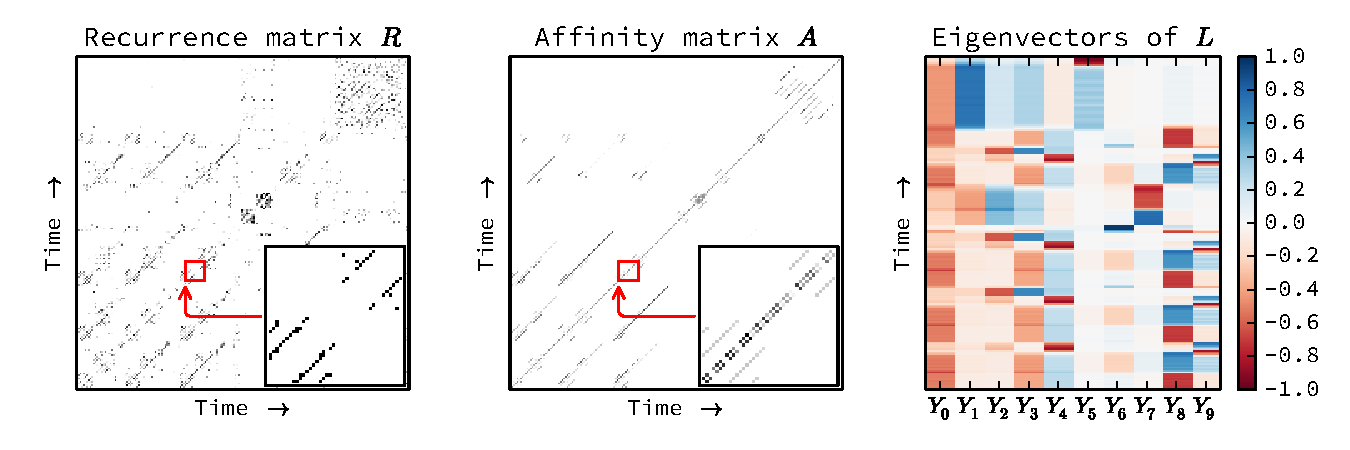
\includegraphics[width=\columnwidth]{figs/recurrence}
\caption{Upper-left: the recurrence matrix $R$ for \emph{The Beatles -- Come
Together}; upper-right: the filtered $R'$; lower-left: a close-up of augmented
recurrence matrix $A$ (first 140 samples); 
lower-right the first 10 basis features, ordered bottom-to-top.  
The first four rows encode the primary structural components.\label{recurrence}}
\end{figure}

 
\begin{figure*}
\centering
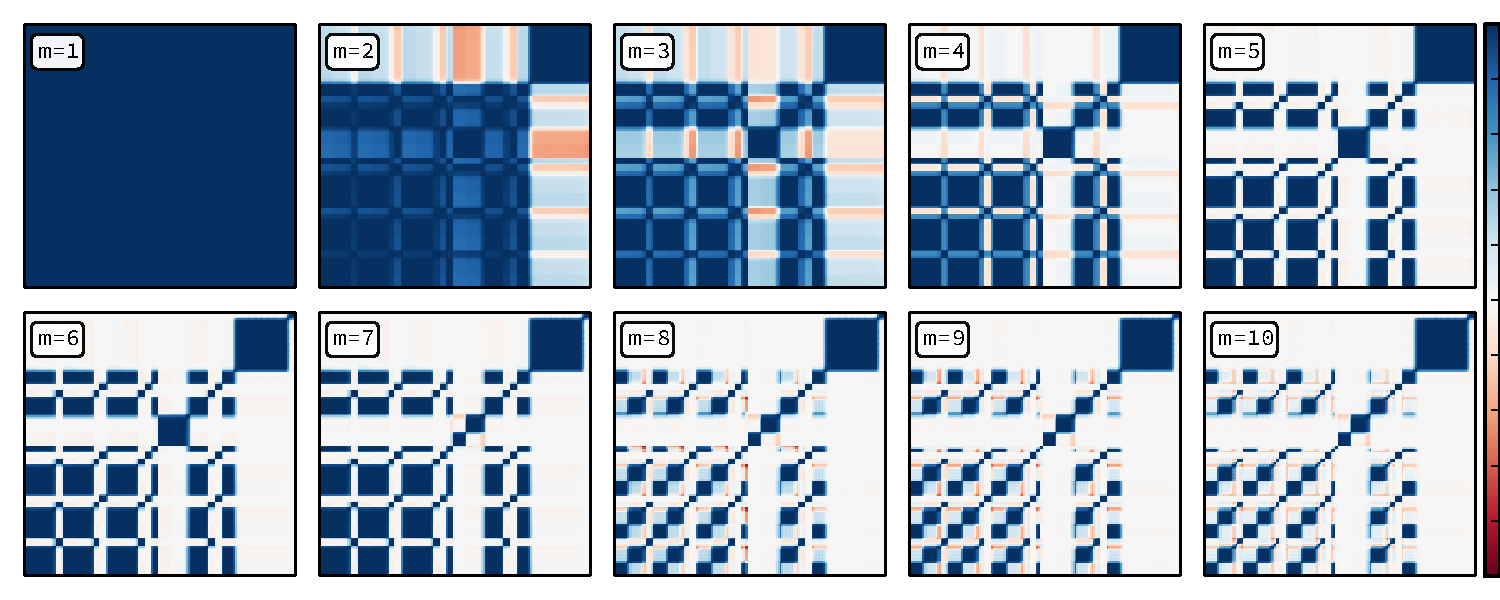
\includegraphics[width=\textwidth]{figs/lowrank}
\caption{Pairwise frame similarity using the first $5$ components for \emph{The Beatles -- Come Together}.  The first
(trivial) component ($m=1$) captures the entire song, and the second ($m=2$) separates the solo and outro from the
rest of the song.  Subsequent refinements separate the verses and refrains, and then encode internal structure.\label{lowrank}}
\end{figure*}

\section{Algorithms}

\subsection{Change-point detection}

\begin{algorithm}
\caption{Change-point detection\label{cpd}}
\begin{algorithmic}[1]
\REQUIRE{Repetition features $Y \in \R^{M \times n}$, $2 \leq k_\text{min} < k_\text{max}$}
\ENSURE{Boundaries $B^*$, number of segment labels $m^*$}\\
{\sc CPD}$(Y, k_\text{min}, k_\text{max})$
    \STATE{$B^* \leftarrow \emptyset$}
    \FOR{$m \leftarrow 1, 2, \ldots, M$}
        \STATE{Run spectral $k$-means on $Y^{(m)}$ with $k=m$}
        \STATE{Let $c_t$ be the cluster containing sample $t$}
        \STATE{$B \leftarrow \{t \given c_t \neq c_{t+1}\}$}
        \IF{$B^* = \emptyset$ or $k_\text{min} \leq |B| + 1 \leq k_\text{max}$} 
        \STATE{$B^* \leftarrow B, \quad m^* \leftarrow m$}
        \ENDIF
    \ENDFOR
    \RETURN{$B^*, m^*$}
\end{algorithmic}
\end{algorithm}

\subsection{Structure annotation}

\begin{algorithm}
\caption{Laplacian structural segmentation\label{lss}}
\begin{algorithmic}[1]
\REQUIRE{ Features: $X \in \R^{d\times n}$\\
maximum number of segment types: $M$\\
bounds on the number of segments: $2 \leq k_\text{min} < k_\text{max}$}
\ENSURE{Segment boundaries $B$, labels $C$}\\
{\sc LSS}$(X, k_\text{min}, k_\text{max}$)
\STATE{$R' \leftarrow $ filtered recurrence matrix of $X$ (\Cref{filtered-rep})}
\STATE{$A \leftarrow R' + \diag_{+1}(\one) + \diag_{-1}(\one)$}
\STATE{$L \leftarrow I - D^{-1} A$}
\STATE{$Y \leftarrow$ bottom $M$ eigenvectors of $L$}
\STATE{$B \leftarrow \text{\sc CPD}(Y, k_\text{min}, k_\text{max})$}
\COMMENT{\Cref{cpd}}
\STATE{$S_i \leftarrow$ mean of $Y^{m}$ over $[B_i, B_{i+1})$}
\STATE{Run $k$-means on $S$ with $k=m$}
\STATE{Let $C_i$ be the cluster containing the $i$th segment}
\RETURN{$B, C$}
\end{algorithmic}
\end{algorithm}

% For each m in 2 .. M:
% m <- argmax gap
% compute segment centroids over boundaries[m], and cluster by k-means with k=m
% return boundary times and segment labels

\section{Experiments}

\subsection{Data}

\subsection{Implementation}

\subsection{Results}

\section{Discussion}

\bibliography{refs}

\end{document}
